% 2008 年新课标卷理科第 24 题：供作图画图用的坐标纸（原页给出空白网格与坐标轴）。
% 来源 PDF：gaokaomath-src/普通高考/2008/2008新课标理(海南,宁夏).pdf
% SHA-256：e16be52b93c241bf45c4d6441855b577407007de032d2e902f11442c06ef66ec
% 原页：2008新课标理(海南,宁夏).pdf 第 2 页（A3 三栏）第 3 栏，书页码 468。
% 绘制依据：按原页画 18×20 的方格坐标纸，坐标轴取在距左边 7 格、距上边 10 格处，
%   并在原点右侧第 2 格处标 1、原点上方第 2 格处标 1。
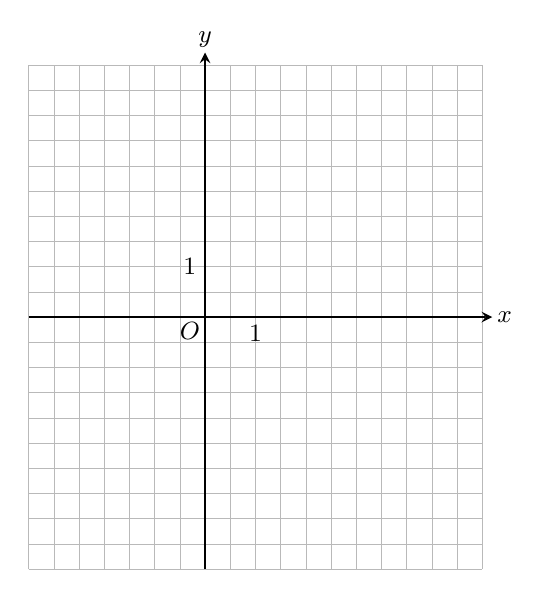
\begin{tikzpicture}[scale=0.32, semithick, every node/.style={inner sep=1.5pt, font=\small}]
  % 坐标纸网格
  \draw[step=1, gray!55, very thin] (0,0) grid (18,20);

  % 坐标轴（x 轴在 y=10，y 轴在 x=7）
  \draw[->,>=stealth, line width=0.7pt] (0,10) -- (18.4,10) node[right] {$x$};
  \draw[->,>=stealth, line width=0.7pt] (7,0) -- (7,20.5) node[above] {$y$};
  \node[below left] at (7,10) {$O$};
  \node[below] at (9,9.85) {$1$};
  \node[left] at (6.85,12) {$1$};
\end{tikzpicture}
